\documentclass[tikz,border=8pt]{standalone}
\usepackage{amsmath,amssymb}
\usepackage{tikz}
\usetikzlibrary{calc}

\begin{document}
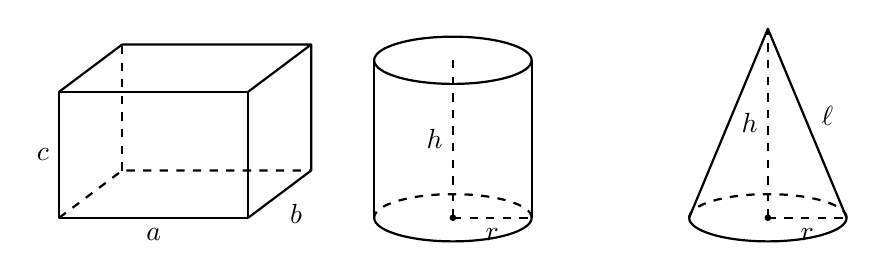
\begin{tikzpicture}[thick, line join=round]
  % Dikdörtgenler prizması
  \begin{scope}
    \def\a{2.4} \def\b{1.6} \def\c{1.2}
    \coordinate (d) at (0.8,0.6);
    \draw (0,0) rectangle (\a,\b);
    \draw (0,\b) -- ++(d) -- ++(\a,0) -- (\a,\b);
    \draw (\a,0) -- ++(d) -- ++(0,\b);
    \draw[dashed] (0,0) -- ++(d) -- ++(\a,0);
    \draw[dashed] ($(0,0)+(d)$) -- ++(0,\b);
    \node[below] at (\a/2,0) {$a$};
    \node[left]  at (0,\b/2) {$c$};
    \node[below right] at ($(\a,0)+0.5*(d)$) {$b$};
  \end{scope}

  % Silindir
  \begin{scope}[xshift=5cm]
    \draw (0,2) ellipse (1 and 0.3);
    \draw (-1,0) -- (-1,2) (1,0) -- (1,2);
    \draw (-1,0) arc (180:360:1 and 0.3);
    \draw[dashed] (1,0) arc (0:180:1 and 0.3);
    \draw[dashed] (0,0) -- node[below] {$r$} (1,0);
    \draw[dashed] (0,0) -- node[left] {$h$} (0,2);
    \fill (0,0) circle (1.2pt);
  \end{scope}

  % Koni
  \begin{scope}[xshift=9cm]
    \draw (-1,0) -- (0,2.4) -- (1,0);
    \draw (-1,0) arc (180:360:1 and 0.3);
    \draw[dashed] (1,0) arc (0:180:1 and 0.3);
    \draw[dashed] (0,0) -- node[below] {$r$} (1,0);
    \draw[dashed] (0,0) -- node[left] {$h$} (0,2.4);
    \node[right] at (0.55,1.3) {$\ell$};
    \fill (0,0) circle (1.2pt);
  \end{scope}
\end{tikzpicture}
\end{document}
